% NIME 2020 Music Proceedings Template

% Modified November 2024 by Charles Martin
% Modified December 2019 by Joe Wright
% Created August 2019 by Niccolo Granieri
% This is file `music-proceedings-template.tex',

\documentclass{nimemusic}

% Rights management information.
\setcopyright{cc4}
\nimeYear{2024}
\nimeMonth{9}
% \nimeDOI{10.1145/XXXXXXX.XXXXXXX}

% Comment out one of the following lines...
\whichProceedings{Music Proceedings of the International Conference on New Interfaces for Musical Expression}
% \whichProceedings{Workshop Proceedings of the International Conference on New Interfaces for Musical Expression}

% Make sure this is correct for the NIME you are submitting to.
\whichNIME{NIME'25, June 24--27, 2025. The Australian National University, Canberra, Australia.}

\begin{document}

\title{Title: Your NIME Music Performance}

% Author information, leave this blank for the initial submission.
\author{Author One}
\affiliation{%
  \institution{Affilitation}
  \city{City}
  \country{Country}
}

\author{Author Two}
\affiliation{%
  \institution{Another Affilitation}
  \city{City}
  \country{Country}
}

\author{Author Three}
\affiliation{%
  \institution{More Affilitations}
  \city{City}
  \country{Country}
}

% Uncomment this command to define a custom short list of authors.
% \renewcommand{\shortauthors}{One, Two and Three}

% Keywords: use these to describe your work.
\keywords{typical, keywords, fix, these, before, submission}

\maketitle

\section{Program Notes}

Lorem ipsum dolor sit amet, consectetur adipiscing elit. Duis sodales nunc vitae arcu mattis elementum. Praesent neque arcu, tincidunt a blandit ut, molestie vel massa. In vitae augue mollis, venenatis tellus a, lobortis ex. Aliquam erat volutpat. Suspendisse potenti. Nunc faucibus lacus ut est elementum pharetra. Sed lorem quam, tempus at interdum sit amet, bibendum ut sem. Ut at neque non velit fermentum laoreet. Vivamus ut aliquet velit. Nam id nunc id ante semper dignissim eget eget risus. Nullam suscipit malesuada ante in lobortis.

Plus, some citations to articles: \cite{doe2023,
wizard2022, alien2024}.

\begin{figure}[hbt]
  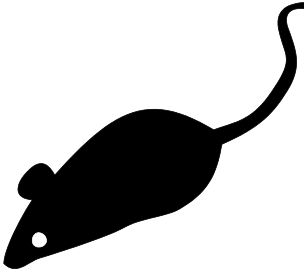
\includegraphics{NIME_Mouse}
  \caption{The NIME Mouse}
\end{figure}

\section{Project Description}

Suspendisse vel pharetra nibh, vel luctus metus. Donec porta dapibus lacinia. Etiam in accumsan enim. Nam vel fermentum libero. Vivamus placerat enim ac sem pharetra cursus. Fusce cursus diam at lacus mattis condimentum. Vestibulum eleifend ante ut ultrices semper. Suspendisse at magna in eros sollicitudin hendrerit eu sed nibh. Integer dapibus felis finibus ornare dignissim. Aliquam semper urna ut purus feugiat vestibulum. In vel nulla volutpat, posuere erat quis, pretium felis. Ut nec tincidunt metus. Fusce libero nunc, mattis vel dignissim non, tempus dapibus nunc. Aliquam enim velit, sagittis non nulla ac, dictum porttitor sapien. Aenean ut volutpat nibh, et porta mi.

Vivamus non purus libero. Orci varius natoque penatibus et magnis dis parturient montes, nascetur ridiculus mus. Nulla a ornare nulla. Proin in convallis libero. Cras ornare pharetra neque quis ultrices. Integer egestas odio convallis orci aliquam, quis tincidunt leo luctus. Duis fringilla leo eget ante ultricies viverra. Quisque elit lacus, egestas vel ultricies quis, eleifend vel purus. Duis eu finibus ex, eu mattis lectus. Duis a laoreet tellus, sed eleifend augue. Sed elementum sem at sapien pellentesque, sit amet varius sapien eleifend. Curabitur ultricies lorem nec dolor ornare, id sodales sapien rutrum.

\section{Technical Notes}

Nulla id dapibus nibh. Suspendisse ultrices dapibus egestas. Sed diam turpis, gravida vitae nibh in, tincidunt hendrerit nulla. Curabitur viverra nibh id lectus volutpat posuere. Fusce tristique condimentum eros, sed mollis ligula euismod sit amet. Proin consectetur dignissim metus, viverra blandit mauris lacinia vel. Vivamus maximus sed elit eu elementum. Nam iaculis vel est vel semper. Nullam pharetra, augue iaculis luctus elementum, urna odio gravida elit, in sagittis ligula magna ac erat.

Suspendisse vel nisl porta, venenatis dui interdum, faucibus risus. Donec congue, dolor quis consequat facilisis, tellus neque lobortis dolor, ullamcorper suscipit turpis massa vitae mauris. Aliquam venenatis augue posuere, pretium turpis dictum, consequat metus. Aenean quis eros enim. Aenean ac magna porttitor, lacinia enim id, facilisis arcu. Donec eleifend mi nec ipsum ultrices posuere. Quisque eu erat venenatis velit dapibus auctor in non ligula. Vestibulum nisl justo, aliquet ut elit a, bibendum pulvinar lectus.

\section{Media Links}

In this section, please provide a list of links to media representations of your submission.

\begin{itemize}
	\item Video: \url{https://www.yournimevideolink.com/younameit}
	\item Audio: \url{https://www.yournimeaudiolink.com/younameit}
\end{itemize}

% The acknowledgements section is optional and can be removed if not needed.
\begin{acks}
The authors would like to thank\ldots
\\
This work was supported by\ldots
\end{acks}

\section*{Ethical Standards}

Please note that an Ethical Standards section is required for all NIME submissions.

This could include information regarding sources of funding, sustainability factors, potential conflicts of interest,  informed consent if the research involved human participants, statement on welfare of animals if the research involved animals, or other ethical factors that are relevant to the work.

% bibliography style
\bibliographystyle{ACM-Reference-Format}
% reference file
\bibliography{references}
\end{document}
